\def\year{2023}\relax
%File: progress_report.tex
\documentclass[letterpaper]{article} % DO NOT CHANGE THIS
\usepackage{aaai21}  % DO NOT CHANGE THIS
\usepackage{times}  % DO NOT CHANGE THIS
\usepackage{helvet} % DO NOT CHANGE THIS
\usepackage{courier}  % DO NOT CHANGE THIS
\usepackage[hyphens]{url}  % DO NOT CHANGE THIS
\usepackage{graphicx} % DO NOT CHANGE THIS
\urlstyle{rm} % DO NOT CHANGE THIS
\def\UrlFont{\rm}  % DO NOT CHANGE THIS
\usepackage{natbib}  % DO NOT CHANGE THIS AND DO NOT ADD ANY OPTIONS TO IT
\usepackage{caption} % DO NOT CHANGE THIS AND DO NOT ADD ANY OPTIONS TO IT
\frenchspacing  % DO NOT CHANGE THIS
\setlength{\pdfpagewidth}{8.5in}  % DO NOT CHANGE THIS
\setlength{\pdfpageheight}{11in}  % DO NOT CHANGE THIS
%\nocopyright
%PDF Info Is REQUIRED.
% For /Author, add all authors within the parentheses, separated by commas. No accents or commands.
% For /Title, add Title in Mixed Case. No accents or commands. Retain the parentheses.

\pdfinfo{
/Title QWOP Bot Progress Report
/Author Matthew Oros, Sonny Smith, Michael Terekhov
/TemplateVersion (2021.2)
} %Leave this
% /Title ()
% Put your actual complete title (no codes, scripts, shortcuts, or LaTeX commands) within the parentheses in mixed case
% Leave the space between \Title and the beginning parenthesis alone
% /Author ()
% Put your actual complete list of authors (no codes, scripts, shortcuts, or LaTeX commands) within the parentheses in mixed case.
% Each author should be only by a comma. If the name contains accents, remove them. If there are any LaTeX commands,
% remove them.

% DISALLOWED PACKAGES
% \usepackage{authblk} -- This package is specifically forbidden
% \usepackage{balance} -- This package is specifically forbidden
% \usepackage{color (if used in text)
% \usepackage{CJK} -- This package is specifically forbidden
% \usepackage{float} -- This package is specifically forbidden
% \usepackage{flushend} -- This package is specifically forbidden
% \usepackage{fontenc} -- This package is specifically forbidden
% \usepackage{fullpage} -- This package is specifically forbidden
% \usepackage{geometry} -- This package is specifically forbidden
% \usepackage{grffile} -- This package is specifically forbidden
% \usepackage{hyperref} -- This package is specifically forbidden
% \usepackage{navigator} -- This package is specifically forbidden
% (or any other package that embeds links such as navigator or hyperref)
% \indentfirst} -- This package is specifically forbidden
% \layout} -- This package is specifically forbidden
% \multicol} -- This package is specifically forbidden
% \nameref} -- This package is specifically forbidden
% \usepackage{savetrees} -- This package is specifically forbidden
% \usepackage{setspace} -- This package is specifically forbidden
% \usepackage{stfloats} -- This package is specifically forbidden
% \usepackage{tabu} -- This package is specifically forbidden
% \usepackage{titlesec} -- This package is specifically forbidden
% \usepackage{tocbibind} -- This package is specifically forbidden
% \usepackage{ulem} -- This package is specifically forbidden
% \usepackage{wrapfig} -- This package is specifically forbidden
% DISALLOWED COMMANDS
% \nocopyright -- Your paper will not be published if you use this command
% \addtolength -- This command may not be used
% \balance -- This command may not be used
% \baselinestretch -- Your paper will not be published if you use this command
% \clearpage -- No page breaks of any kind may be used for the final version of your paper
% \columnsep -- This command may not be used
% \newpage -- No page breaks of any kind may be used for the final version of your paper
% \pagebreak -- No page breaks of any kind may be used for the final version of your paperr
% \pagestyle -- This command may not be used
% \tiny -- This is not an acceptable font size.
% \vspace{- -- No negative value may be used in proximity of a caption, figure, table, section, subsection, subsubsection, or reference
% \vskip{- -- No negative value may be used to alter spacing above or below a caption, figure, table, section, subsection, subsubsection, or reference

\setcounter{secnumdepth}{0} %May be changed to 1 or 2 if section numbers are desired.

% The file aaai21.sty is the style file for AAAI Press
% proceedings, working notes, and technical reports.
%

% Title

% Your title must be in mixed case, not sentence case.
% That means all verbs (including short verbs like be, is, using,and go),
% nouns, adverbs, adjectives should be capitalized, including both words in hyphenated terms, while
% articles, conjunctions, and prepositions are lower case unless they
% directly follow a colon or long dash

\title{QWOP Bot Progress Report}
\author{
    %Authors
    % All authors must be in the same font size and format.
    Written by Matthew Oros, Sonny Smith, and Michael Terekhov \\ 
}
\affiliations{
    %Afiliationsz
    Baldwin Wallace University\\
    %If you have multiple authors and multiple affiliations
    % use superscripts in text and roman font to identify them.
    %For example,

    % Sunil Issar, \textsuperscript{\rm 2}
    % J. Scott Penberthy, \textsuperscript{\rm 3}
    % George Ferguson,\textsuperscript{\rm 4}
    % Hans Guesgen, \textsuperscript{\rm 5}.
    % Note that the comma should be placed BEFORE the superscript for optimum readability

    275 Eastland Road\\
    Berea, Ohio 44017\\
    % email address must be in roman text type, not monospace or sans serif

    % See more examples next
}
\iffalse
%Example, Single Author, ->> remove \iffalse,\fi and place them surrounding AAAI title to use it
\title{My Publication Title --- Single Author}
\author {
    % Author
    Author Name \\
}

\affiliations{
    Affiliation \\
    Affiliation Line 2 \\
    name@example.com
}
\fi

\iffalse
%Example, Multiple Authors, ->> remove \iffalse,\fi and place them surrounding AAAI title to use it
\title{My Publication Title --- Multiple Authors}
\author {
    % Authors
    First Author Name,\textsuperscript{\rm 1}
    Second Author Name, \textsuperscript{\rm 2}
    Third Author Name \textsuperscript{\rm 1} \\
}
\affiliations {
    % Affiliations
    \textsuperscript{\rm 1} Affiliation 1 \\
    \textsuperscript{\rm 2} Affiliation 2 \\
    firstAuthor@affiliation1.com, secondAuthor@affilation2.com, thirdAuthor@affiliation1.com
}
\fi

\graphicspath{{./img/}}

\begin{document}

\maketitle

\begin{abstract}

QWOP is a challenging 2-dimensional game where the goal is to make the main character walk/run to the right as far as possible without falling. The game's difficulty lies in its physics simulation, which makes movements hard to predict and requires a quick reaction time as well as an understanding of how the combinations of key presses translate to a desired movement on the screen. The character is controlled using four keyboard keys: Q, W, O, and P. Q and W control the thighs, and O and P control the knees by either rotating the joints one way or the other. As soon as an upper-body limb contacts the flat ground, the game is over and restarted. The score of the game is based on the distance traveled by the character.

\par In this project, we propose a simulation that allows an agent to learn to control the character and play the game of QWOP. Two main implementations are considered and attempted, both based on neural networks. The first method is a genetic algorithm approach to learning, while the second approach is a deep Q-learning method.

\par The genetic approach is inspired by natural selection where the best performers get to reproduce and spread their genetic information to their offspring. The new population then replaces the old one and plays the game again. This process is repeated until the agents play the game to a satisfactory level.

\par The deep Q-learning approach is a powerful reinforcement learning method that approximates the Q-function, which measures the expected reward of taking a certain action in a given state. By combining the benefits of deep learning and reinforcement learning, the deep Q-learning approach can learn to make optimal decisions in a wide range of environments, even in situations where the optimal policy is not known in advance or labeled data is not available.

\end{abstract}

\begin{figure}[h]
\caption{The original browser-game QWOP}
\centering
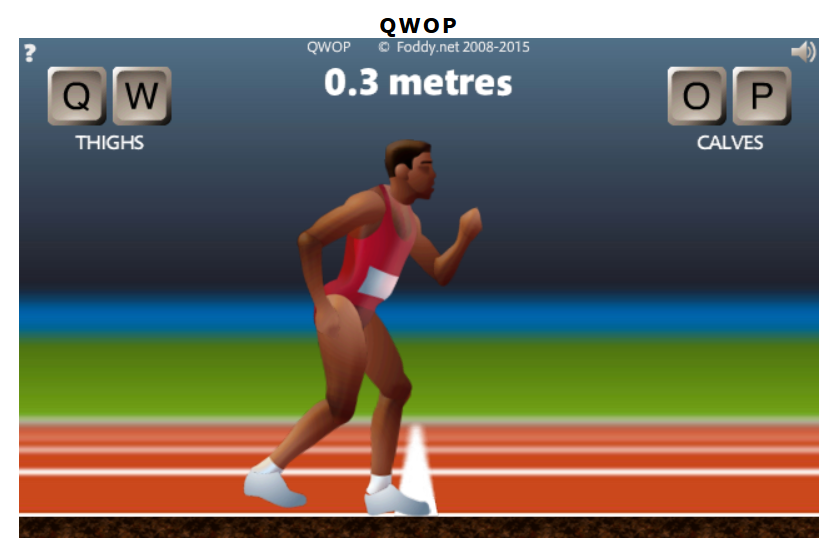
\includegraphics[width=7cm]{qwop.png}
\end{figure}

\section{Proposed Implementation}

The proposal of the simulation is an agent that is able to learn on its own to control the character to play the game of QWOP. Two main implementations that will be considered and attempted will both be based on neural networks. The first method is a genetic algorithm approach to learning while the second approach will be a deep Q method of learning. A neural network is chosen for both methods as deep neural networks have successfully reproduced highly-detailed human movements including walking, running, cartwheel, and flipping \cite{2018-TOG-deepMimic}.

\section{Consideration of Backpropagation}

A traditional method of training a neural network is to use a method called backpropagation. Backpropagation is done by providing the network with input data and labeled output data where the term labeled refers to the desired output of the given input. It is to be noted that the term backpropagation used in this context is referring to the entire learning approach while it can also be used to refer to a step in a different overall learning approach such as deep-q learning. In this context, it is referring to an overall learning approach where backpropagation is the main overall training step. The input is fed forward through the network in its current state and its output is compared to the labeled output. The weights are then adjusted from back to front based on how incorrect the network's output is. 

\par The difficulty with this approach for this domain of problem is that there is no simple method of obtaining such labeled data in this problem. The game of QWOP is difficult for humans and such the goal of the simulation is for the learning process to generate a solution from its fitness feedback and environment rather than by example from human playthrough. Thus, the two methods that were chosen incorporate some form of random exploration of the state space to converge on a desired solution.

\section{Genetic Approach}

The genetic approach is inspired by natural selection. In each generation, a specific amount of agents is created and each has a distinct neural network (genes). These genes can be mutated, recombined, and evaluated for fitness. Based on their fitness, individuals are selected for reproduction, which involves combining their genes to create new offspring. The new population then replaces the old one, and the process is repeated until the agents play the game to a satisfactory level.

\par Our approach is based on the simple evolutionary algorithm that is presented in the article \textit{Evolving Controllers for Virtual Creature Locomotion}. As it is described in the article, "An evolutionary algorithm (EA) is a search method modelled on natural evolutionary processes. The search is formulated as an optimization problem - we define a real-valued fitness function the value of which increases with the optimality of the solution candidate. In our case, a solution candidate is a description of a particular locomotion controller and the fitness function is a measure of how far the virtual creature moves over a fixed time during a physically-based simulation"\cite{sanders_lobb_riddle_2003}.

\par The approach that is utilized includes three phases. The first phase is to create 100 agents where each has a distinct neural network. For the first generation, the weights for each neural network are randomly assigned. When the agents are created they perform actions that are based on inputs of their limbs' locations. After the time that is specified passes, the program moves to the second phase. In the second phase, the top 50 performers are chosen based on their fitness function. Then the neural networks of the performers are randomly chosen to create new ones that will be used for the next generation. The process of creating a new neural network involves picking two random top performers, taking their neural networks, and mixing them. The mixing is based on the specified probability, in our case is 50\%. This means that for each specific connection/weight between the layers half of the time the algorithm will choose the connection/weight of neural network $A$ and half of the time of neural network $B$. Mutation probability is also included and is 5\%. A mutation is important in this case since it introduces new genetic material into the population, which can help to avoid premature convergence of the algorithm on a suboptimal solution. It is important to mention that we keep the top five performers for the next generation and create 95 new neural networks based on the top 50 performers. Hence we have 100 neural networks for the next generation. Such technic is called elitism and is useful to preserve the best solutions found throughout all generations. Elitism allows us to build upon the best solutions and converge toward a desirable solution more quickly. The third phase is to create new agents which will have the newly created neural networks and let them play again. The process is repeated until the desirable solution is achieved.

\section{Deep-Q Learning Approach}

The proposed method is based on deep Q-learning, a model-free, bootstrapped, off-policy learning algorithm. This implies that the agent does not require any prior knowledge of the environmental dynamics. The agent learns by interacting with the environment and collecting experience samples. This learning approach is promising as the agent learns to perform various skills through trial-and-error, thus reducing the need for human insight \cite{2018-TOG-deepMimic}. The algorithm constructs estimates of the action-value functions, which represent the expected return of taking each action in a given state, based on previous estimates. This is a bootstrapping process, where one estimate is used to update another. The algorithm also employs an off-policy strategy, where it uses an epsilon-greedy policy to generate actions that explore the state-action space with a probability epsilon and exploit the current best action with a probability 1-epsilon. The data generated by this exploratory policy is used to update a purely greedy policy that maximizes the action-value function. We implement decay into our epsilon based on the considerations made in the article \textit{RBED : Reward Based Epsilon Decay}. We want the epsilon value to decay so that the agent employs more exploitation than exploration as it gains more information about its environment, as "once an agent does have the information it
needs to interact optimally with the environment, allowing it to exploit its knowledge makes more sense" \cite{maroti_2019_rbed}.  

\par The agent possesses various types of memories, namely state memory, new state memory, action memory, reward memory, and terminal memory. These memories are utilized to calculate action-value functions, which are crucial for learning. The terminal memory stores the done flags that indicate when the exploration period ends and the states that need to be updated with the agent's estimates of the action-value Q are passed. To enable the intelligent learning of the agent, batches of memories are used. The batches allow the data to be used for updating the agent's neural network when they are full. By processing the training data in batches, the neural network can update its weights more frequently and efficiently.

\par Mean Squared Error (MSE) is a loss function that is applied. A loss function measures the difference between the estimated action-value function ($Q(s, a)$) and the target action-value function. The target action-value function represents the expected return after taking an action in a given state, and it is computed as the sum of the immediate reward and $\gamma$ (discount factor) times the maximum value for the next state.
$$
\textnormal{target} = \textnormal{reward} + \gamma \cdot \textnormal{max}(Q(s', a'))
$$
The function produces gradients with respect to the weights of the neural network. The gradients are the measures of how much each weight contributes to the overall solution using backpropagation.

\par An optimizer, Adaptive Moment Estimation (Adam), is utilized. Adam uses the gradients of the loss function to update the weights of the neural network that correspond to the global solution. Adam knows in which direction the weights should be nudged by calculating the first and second moments of the gradient from the loss function. The first moment is the moving average of the gradients. The second movement is the moving average of the squared gradients. Adam then adjusts the learning rate for each weight based on these moments, making it larger for weights with low variance, meaning the gradients that are consistent and stable, and smaller for weights with high variance, meaning the gradients are more volatile and unpredictable. This way, Adam can find a good balance between exploring and exploiting the search space and converge faster to a minimum of the loss function.

\section{Current Progress}

In order to create a suitable learning environment for the agent, the original game was reimplemented. The original game is browser-based and would require interfacing code to grab relevant data and to simulate key presses. The logistics of this are not relevant to the desired outcome or exploratory process of the project and thus the approach of re-implementation of the game was chosen.

\par The programming language that was chosen was Python. Python was chosen due to its simplicity, flexibility, and plentiful collection of libraries, especially related to machine learning. For the simulation itself the graphics library chosen is Raylib. Raylib is a native C library but has various bindings to other languages such as Python. It was chosen due to its simplicity where it is not a graphics engine but rather abstracts OpenGl drawing calls to functions. This helps to decouple the simulation from the graphics. The physics library chosen is PyMunk. It is a simple 2D physics library where physics bodies are created with certain shapes and properties and added to a simulation space. PyMunk was also chosen for its simplicity and flexibility.

\par The initial progress on the project started with a basic simulation of physics bodies where the joints that connect them were actuated by a key press. This basic simulation later evolved to create legs and then hips, and then the upper body. Various tweaks were needed to produce a correct feeling simulation based on the original game. In order to accomplish this, the ability to directly control the character with the keyboard was added even though it would not be used in the final result as the simulated agent would be controlling the character. 

\begin{figure}[h]
\caption{A single physics-simulated character}
\centering
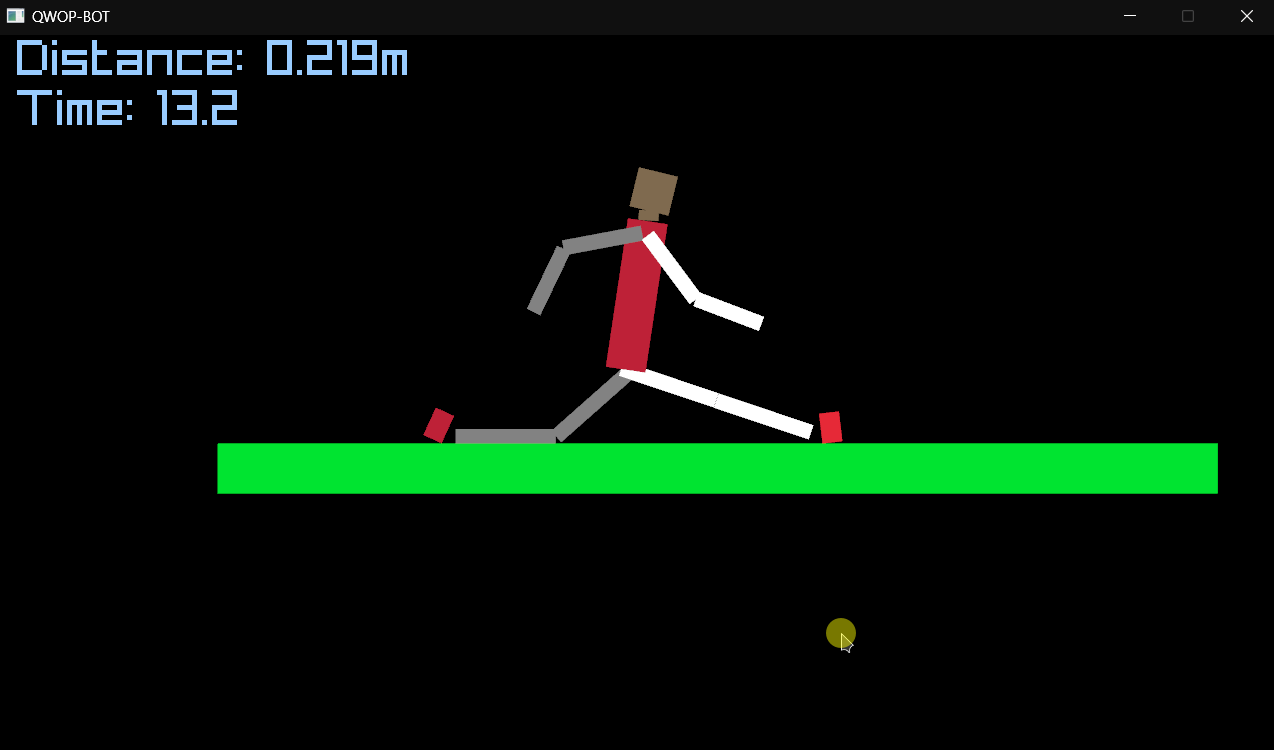
\includegraphics[width=7cm]{character.png}
\end{figure}

\par Once the progress on the physically-simulated character was acceptable, work begun on creating a neural network. The neural network was originally created without use of any libraries. A neural network consists of input neurons that connect to hidden neurons which then connect to output neurons. The strength of the connections between neurons are called weights. Each neuron accepts a single or multiple floating point values which then get summed and normalized using an activation function. The activation function chosen was the sigmoid function as it is very common choice. Which is defined as:
$$
S(x)=\frac{1}{1+e^{-x}}
$$
\par In order to utilize a neural network, the inputs that are fed to the network must be determined. These inputs would denote which aspects of the environment the agent would be informed about. If too little information is forwarded to the network, then it may not be able to converge on an acceptable solution. If too much data is sent, the network may also have difficulty converging with having to weight the numerous inputs. The current implementation sends the global x and y positions of each limb to the network. We hypothesize that this would give the network enough information to determine how it should move its limbs when in a certain physical configuration.

\par Initial work was made on an early termination condition where if certain upper-body limbs contact the ground then the simulation ends for that particular character and its reward function is adjusted accordingly. An advantage of early termination is that it can function as a curating mechanism that biases the data distribution in favor of samples that may be more relevant for a given task \cite{2018-TOG-deepMimic}.

\section{Implementation of Genetic Algorithm}

In order to maximize the efficiency of learning for the genetic algorithm portion of the project, it is important to simulate many generations at a decent speed. To maximize the throughput of the simulations, each generation is simulated in batches where each batch is simulated all at once. For example, a generation of 100 characters is split into 10 sub-generations each containing 10 characters. These characters are all simulated at the same time. This is able to be done easily as PyMunk (the physics library used) is able to simulate multiple isolated simulation spaces. Since the graphics and physics simulation is decoupled, this allows us to visualize all 10 characters in the same sub-generation while they are all actually being simulated in their own simulation space, not influencing each other.

\begin{figure}[h]
\caption{A simulated batch of characters during a sub-generation}
\centering
\includegraphics[width=7cm]{many.png}
\end{figure}

\par The number of characters could be increased for the sub-generation but there is a speed limitation where it would reach a point where the number of characters would slow down the simulation thus negating the added benefit of parallelism.

\section{Problems Encountered and Avoided}

\subsection{Environment}
Throughout development, several problems/difficulties were encountered along the way. First, we had to understand the library that we used to develop a physical character and the environment that it would be in. The first difficulty that we had on the way was figuring out how the libraries that we used to build the character and the environment worked. To create a character, we had to figure out the limits and capabilities of these libraries. To create a character and the environment, we had to figure out how to set up physics, how to create a graphical object, how to give the object physics, how to connect this object with other objects, and how to give them muscles so it can be controllable. 

\subsection{Agent}

The next difficulty we encountered is the structure of the neural network for agents. The difficulty involved choosing how many input nodes were needed, what kind of data will be used for the neural network, and how many hidden layers were needed. Eventually, we deiced to move forward with 24 input nodes which would take in all the x and y positions of the limbs. 

\par The second difficulty concerning the agent was setting up the collision detection. The initial idea was to have collision detection in the environment so that when specific objects collide inside of it, we would get some type of output. The approach turned out to be inappropriate as we progressed forward since we needed to know which agent had contact with the ground. The fix to the problem was to include collision detection inside of the agent class from which each agent was created. That way each agent had its own collision detection, which indicates when the agent touched the ground with its upper body.

\subsection{Simulation Time}

\par An unexpected issue during development was the use of real-world clock time in areas of the simulation. The learning process of the simulation can take numerous iterations, especially for the genetic algorithm to converge on a satisfactory result. Thus a method for increasing the simulation rate was implemented. However, since real-world clock time was used, this resulted in unexpected behavior in multiple area of the application. One example is the time for each generation. Each generation would last three seconds after the maximum distance that was achieved by an one character has not changed. However, when the simulation rate was increased this timing became inaccurate. All time-related code was converted to a simulation time which has no relation to real-world time. This allowed us to increase the rate of the simulation while maintaining the exact same same results as if it were run at a slower, more normal looking rate.

\section{Visualization}

\par To collect data from our program, we initially implemented the ability to save the program's current state as a JSON file. As we further developed our program, we expanded the save functionality to separate the data of each generation that was created. The JSON that we save includes the color of each runner, the bias values of the neural network, and the fitness value of the runners. We decided to utilize the Pandas Python library to visualize our data, as we are already working with Python for our program, and we have experience using Pandas. The JSON files are imported into the visualization program where they are concatenated into a single data frame. It is not useful to visualize the network biases, so they are dropped from the data frame. The visualizations that we intend to use include a histogram of the fitness values of each of the runners in a given generation (Figure 4), a graph of the average fitness values for each generation of runners (Figure 5), and a dual-axis graph that shows the fitness and epsilon values for each runner.

\begin{figure}[h]
\caption
\centering
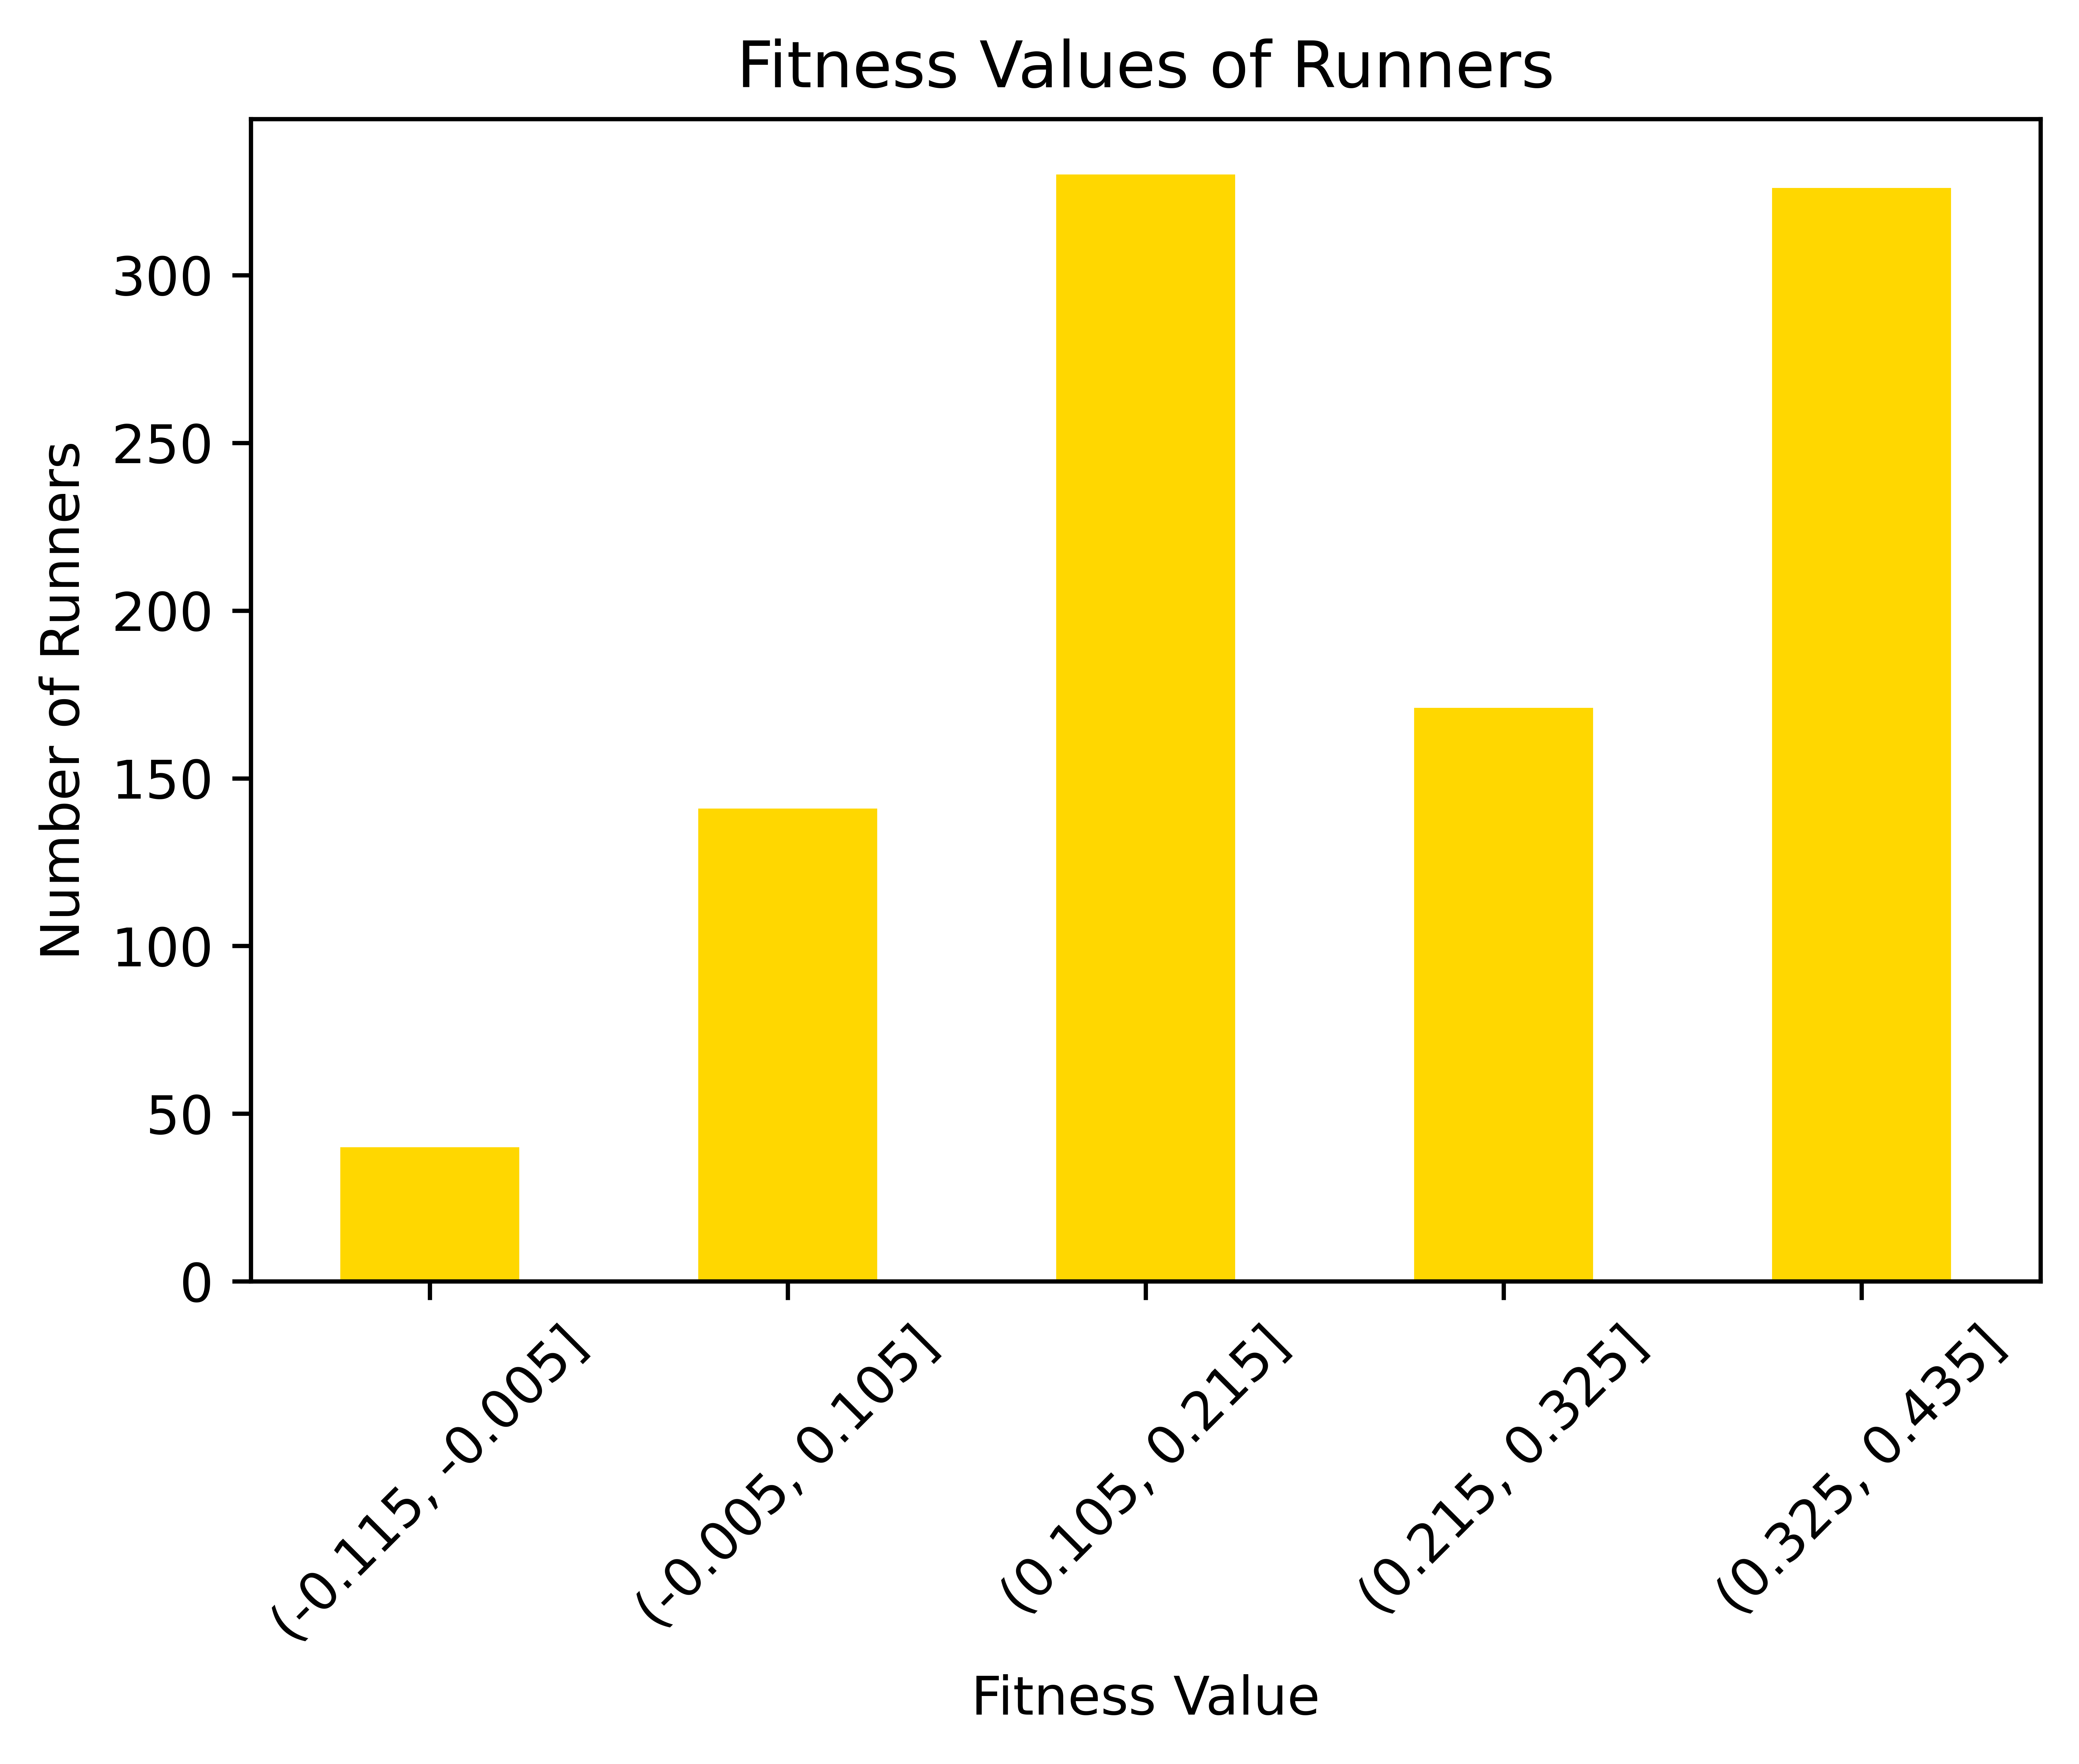
\includegraphics[width=7cm]{fitness_dist.png}
\end{figure}

\begin{figure}[h]
\caption
\centering
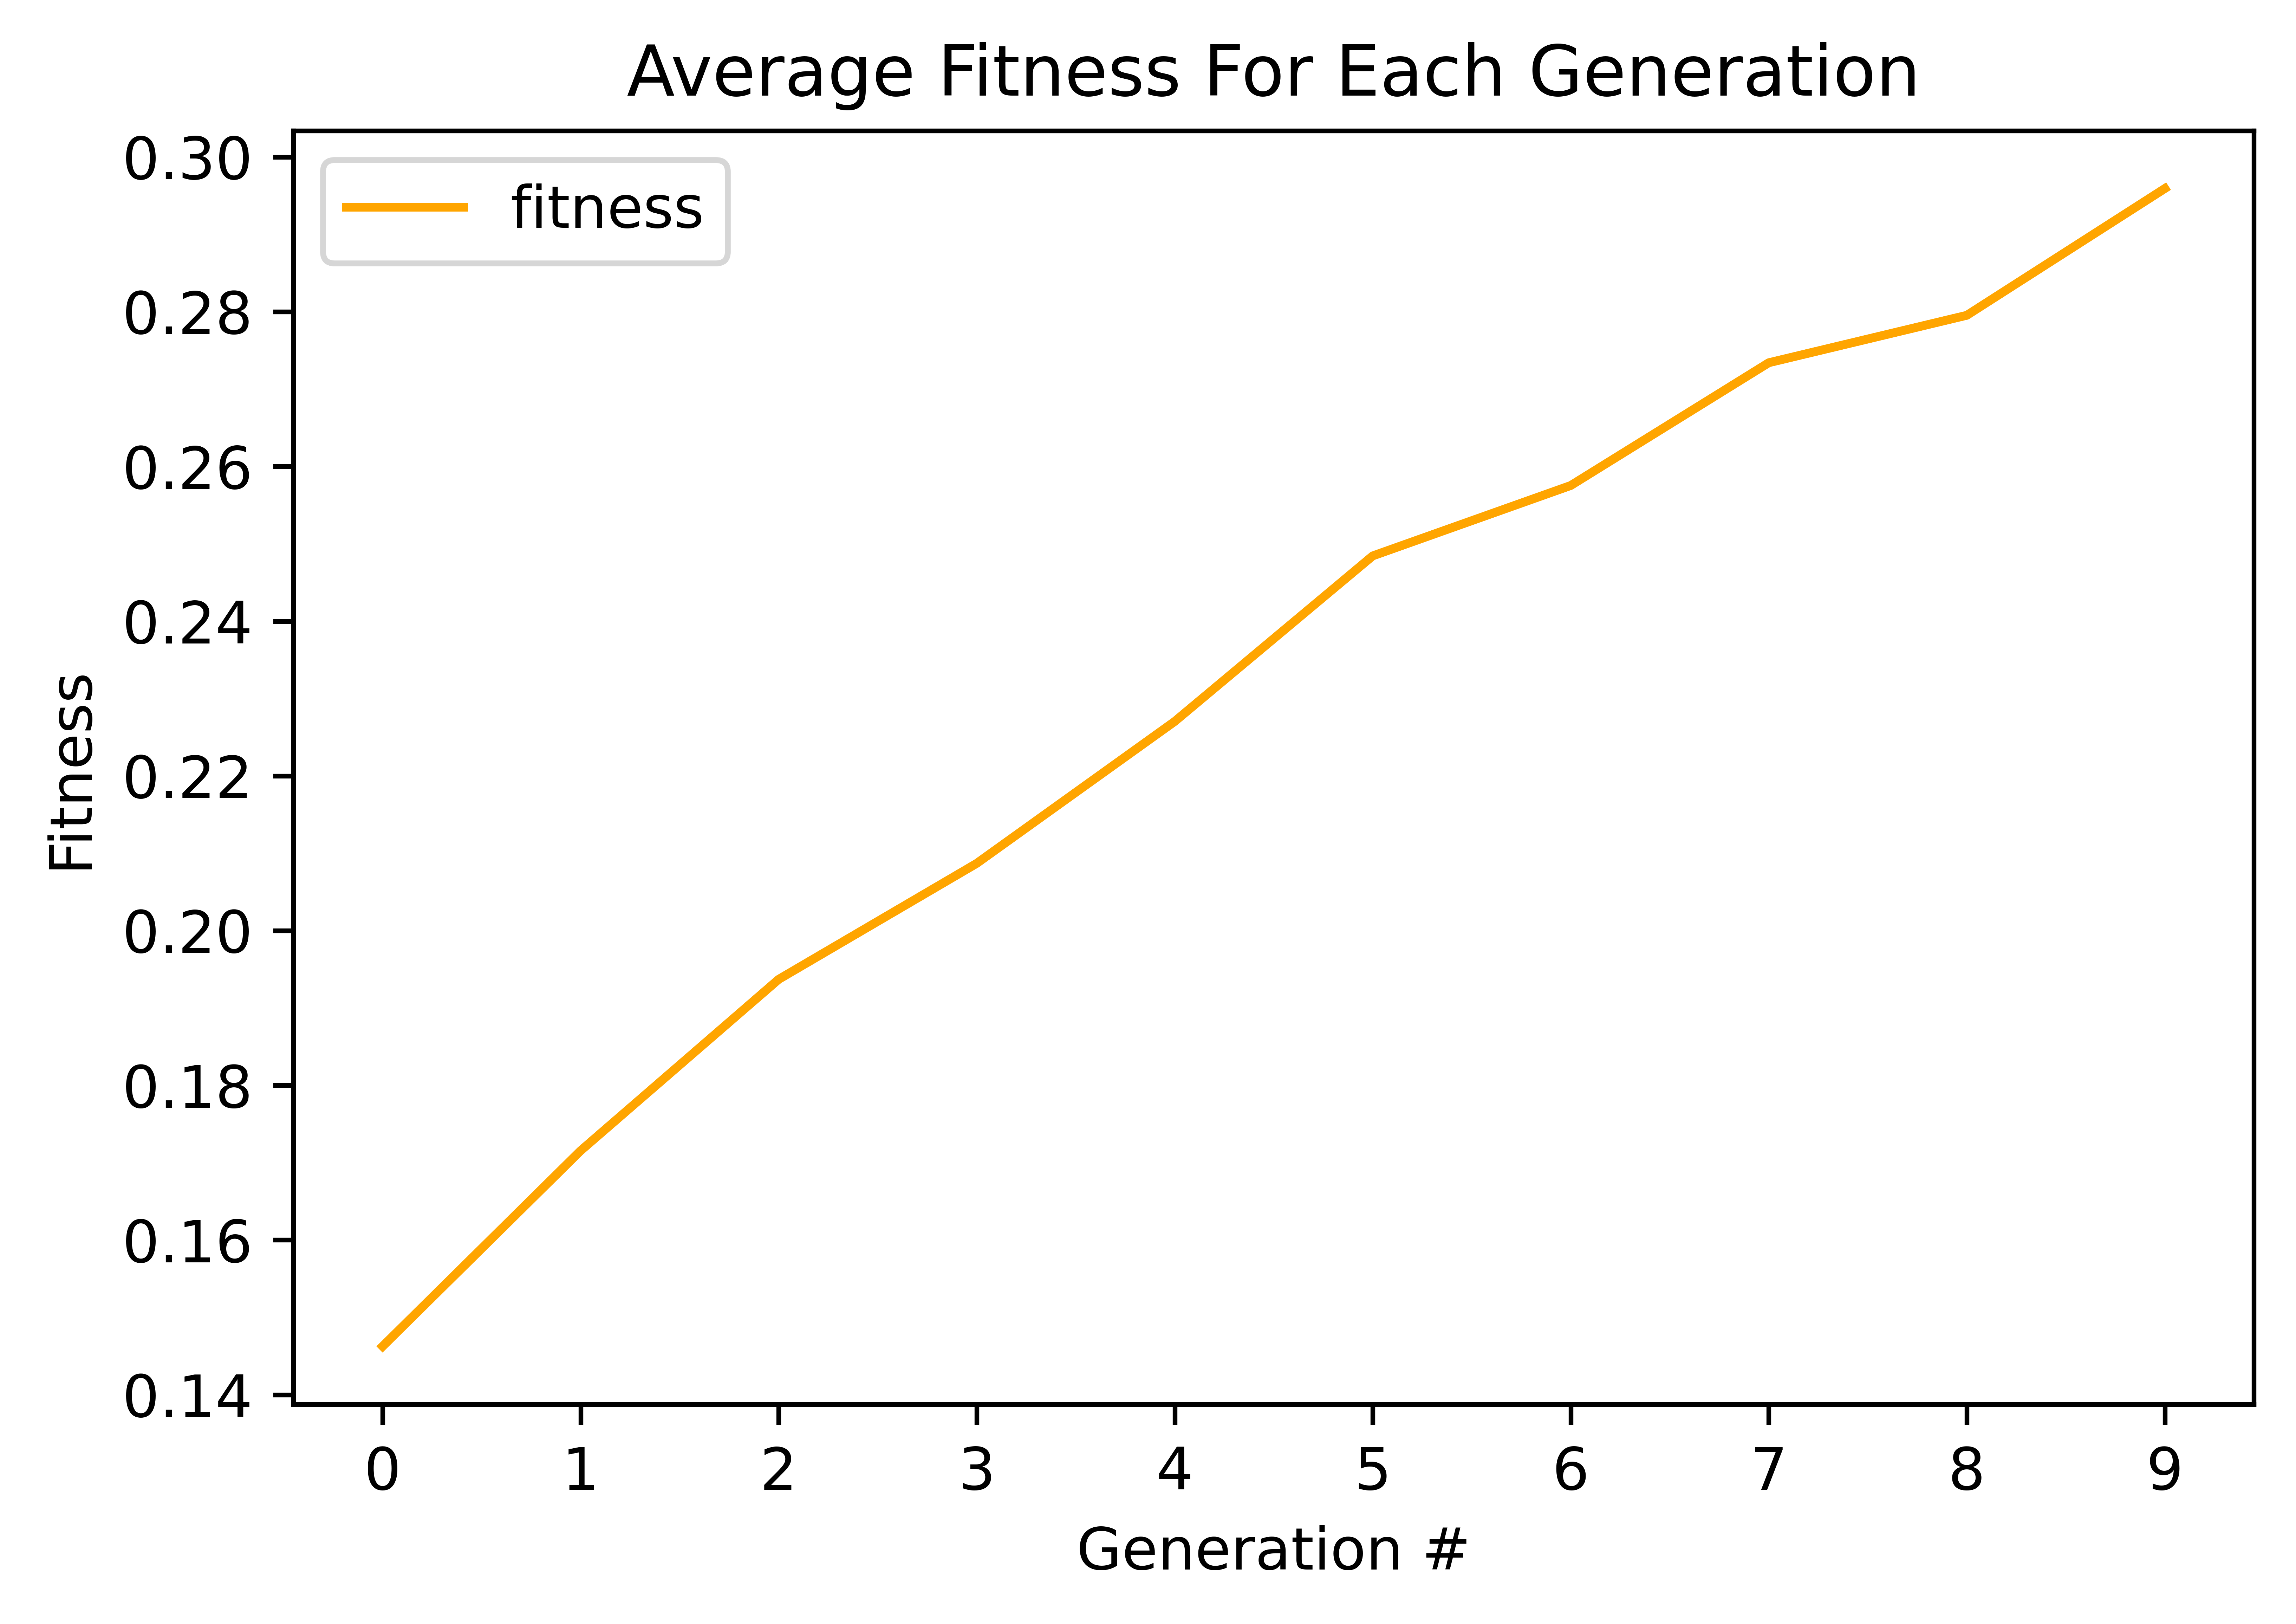
\includegraphics[width=7cm]{avg_fitness_per_gen.png}
\end{figure}


\section{Future Considerations}

Some future considerations for the inputs of the neural network would be to send information regarding the velocity of the character. This might better inform the network. However, it may not be necessary to input velocity for each individual limb and so an average velocity or velocity of just the center of mass might be sufficient. However, this could only be determined through experimentation. Another consideration is that we could have explored a niching evolutionary algorithm like the one described in the article Evolving Controllers for Virtual Creature Locomotion. Such an algorithm could maintain the genetic variation after several generations \cite{sanders_lobb_riddle_2003}.  

\par Another idea might be to have a memory neuron which would be an output neuron whose output is connected to an input neuron. This could potentially allow for the network to retain some type of memory about its computational state. This may be a helpful addition as the problem being solved is highly temporal and so the ability for the network to retain some kind of information about the previous frame to the next could prove to be beneficial.

\bibliography{references.bib}

\end{document}
